\newpage
\subsubsection{UC2 - Addestramento del predittore}
\label{sssec:uc2}

\begin{figure}[h!]
  \begin{center}
    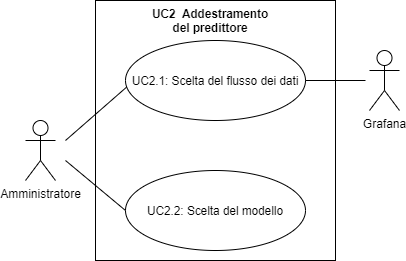
\includegraphics[width=10cm]{uc2.png}\\
    \caption{UC2 - Addestramento del predittore}%
    \label{fig:uc2}
  \end{center}
\end{figure}

\begin{description}
  \item[Attore primario]: Utente amministratore.
  \item[Attore secondario]: Grafana.
  \item[Descrizione:] L'amministratore seleziona un flusso di dati presente in Grafana e il plug-in grazie allo storico dei dati di quel flusso addestara un predittore, utilizzando un modello.
  \item[Precondizione:] L'amministratore ha creato un pannello del plug-in e sa che tipo di modello di machine learning va utilizzato.
  \item[Scenario principale:]
  \begin{enumerate}
    \item L'amministratore sceglie su che dati, tra quelli disponibili in Grafana, compiere l'addestramento (UC2.1);
    \item L'amministratore sceglie un modello da utlizzare (UC2.2).
  \end{enumerate}
  \item[Postcondizione:] Il plug-in ha generato il predittore ed ora è pronto a fare previsioni sui dati.
\end{description}

\paragraph{UC2.1 - Scelta del flusso dei dati}
\label{sssec:uc2.1}
\begin{description}
  \item[Attore primario:] Utente amministratore.
  \item[Descrizione:] L'amministratore sceglie un determinato flusso presente in Grafana.
  \item[Precondizione:] L'amministratore ha creato un pannello del plug-in;
  \item[Scenario principale:] L'amministratore identifica il flusso di dati.
  \item[Postcondizione:] L'amministratore ha scelto un flusso di dati.
\end{description}

\paragraph{UC2.2 - Scelta del modello}
\label{sssec:uc2.2}
\begin{description}
  \item[Attore primario:] Utente amministratore.
  \item[Descrizione:] L'amministratore sceglie un modello da applicare ai dati tra SVM, RL o Rete Neurale.
  \item[Precondizione:] L'amministratore ha scelto un flusso di dati (UC2.1).
  \item[Scenario principale:] L'amministratore deve scegliere un modello tra SVM, RL o Rete Neurale.
  \item[Postcondizione:] L'amministratore ha scelto il modello per l'addestramento.
\end{description}
